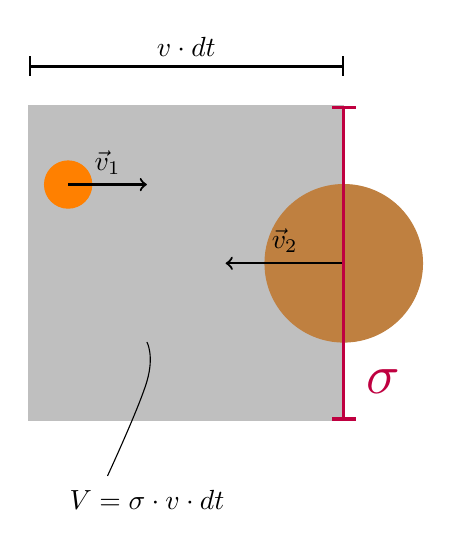
\begin{tikzpicture}

\draw [fill, lightgray] (-1.5,2) rectangle (2.5,-2) node (v3) {};
\draw  [fill, brown](2.5,0) node (v2) {} circle (1);
\draw  [fill, orange](-1,1) node (v1) {} circle (0.3);
\draw [->, thick] (v1.center) -- (0,1) node [midway, above]{$\vec{v}_1$};
\draw [->, thick]  (v2.center) -- (1,0) node [midway, above]{$\vec{v}_2$};
\draw [|-|, very thick, purple](2.5,2) -- (v3.center);
\node [scale=2] at (3,-1.5) [purple]{$\sigma$};
\draw [|-|, thick] (-1.5,2.5) -- (2.5,2.5) node [midway, above]{$v\cdot dt$};
\node at (0,-3) {$V=\sigma\cdot v\cdot dt$};
\draw  plot[smooth, tension=.7] coordinates {(0,-1) (0,-1.5) (-0.5,-2.7)};
\end{tikzpicture}